% Options for packages loaded elsewhere
\PassOptionsToPackage{unicode}{hyperref}
\PassOptionsToPackage{hyphens}{url}
%
\documentclass[
  english,
  man]{apa6}
\usepackage{lmodern}
\usepackage{amssymb,amsmath}
\usepackage{ifxetex,ifluatex}
\ifnum 0\ifxetex 1\fi\ifluatex 1\fi=0 % if pdftex
  \usepackage[T1]{fontenc}
  \usepackage[utf8]{inputenc}
  \usepackage{textcomp} % provide euro and other symbols
\else % if luatex or xetex
  \usepackage{unicode-math}
  \defaultfontfeatures{Scale=MatchLowercase}
  \defaultfontfeatures[\rmfamily]{Ligatures=TeX,Scale=1}
\fi
% Use upquote if available, for straight quotes in verbatim environments
\IfFileExists{upquote.sty}{\usepackage{upquote}}{}
\IfFileExists{microtype.sty}{% use microtype if available
  \usepackage[]{microtype}
  \UseMicrotypeSet[protrusion]{basicmath} % disable protrusion for tt fonts
}{}
\makeatletter
\@ifundefined{KOMAClassName}{% if non-KOMA class
  \IfFileExists{parskip.sty}{%
    \usepackage{parskip}
  }{% else
    \setlength{\parindent}{0pt}
    \setlength{\parskip}{6pt plus 2pt minus 1pt}}
}{% if KOMA class
  \KOMAoptions{parskip=half}}
\makeatother
\usepackage{xcolor}
\IfFileExists{xurl.sty}{\usepackage{xurl}}{} % add URL line breaks if available
\IfFileExists{bookmark.sty}{\usepackage{bookmark}}{\usepackage{hyperref}}
\hypersetup{
  pdftitle={Absence pop-out without task experience},
  pdfauthor={Matan Mazor1 \& Stephen M. Fleming1,2,3},
  pdflang={en-EN},
  hidelinks,
  pdfcreator={LaTeX via pandoc}}
\urlstyle{same} % disable monospaced font for URLs
\usepackage{graphicx,grffile}
\makeatletter
\def\maxwidth{\ifdim\Gin@nat@width>\linewidth\linewidth\else\Gin@nat@width\fi}
\def\maxheight{\ifdim\Gin@nat@height>\textheight\textheight\else\Gin@nat@height\fi}
\makeatother
% Scale images if necessary, so that they will not overflow the page
% margins by default, and it is still possible to overwrite the defaults
% using explicit options in \includegraphics[width, height, ...]{}
\setkeys{Gin}{width=\maxwidth,height=\maxheight,keepaspectratio}
% Set default figure placement to htbp
\makeatletter
\def\fps@figure{htbp}
\makeatother
\setlength{\emergencystretch}{3em} % prevent overfull lines
\providecommand{\tightlist}{%
  \setlength{\itemsep}{0pt}\setlength{\parskip}{0pt}}
\setcounter{secnumdepth}{-\maxdimen} % remove section numbering
% Make \paragraph and \subparagraph free-standing
\ifx\paragraph\undefined\else
  \let\oldparagraph\paragraph
  \renewcommand{\paragraph}[1]{\oldparagraph{#1}\mbox{}}
\fi
\ifx\subparagraph\undefined\else
  \let\oldsubparagraph\subparagraph
  \renewcommand{\subparagraph}[1]{\oldsubparagraph{#1}\mbox{}}
\fi
% Manuscript styling
\usepackage{upgreek}
\captionsetup{font=singlespacing,justification=justified}

% Table formatting
\usepackage{longtable}
\usepackage{lscape}
% \usepackage[counterclockwise]{rotating}   % Landscape page setup for large tables
\usepackage{multirow}		% Table styling
\usepackage{tabularx}		% Control Column width
\usepackage[flushleft]{threeparttable}	% Allows for three part tables with a specified notes section
\usepackage{threeparttablex}            % Lets threeparttable work with longtable

% Create new environments so endfloat can handle them
% \newenvironment{ltable}
%   {\begin{landscape}\begin{center}\begin{threeparttable}}
%   {\end{threeparttable}\end{center}\end{landscape}}
\newenvironment{lltable}{\begin{landscape}\begin{center}\begin{ThreePartTable}}{\end{ThreePartTable}\end{center}\end{landscape}}

% Enables adjusting longtable caption width to table width
% Solution found at http://golatex.de/longtable-mit-caption-so-breit-wie-die-tabelle-t15767.html
\makeatletter
\newcommand\LastLTentrywidth{1em}
\newlength\longtablewidth
\setlength{\longtablewidth}{1in}
\newcommand{\getlongtablewidth}{\begingroup \ifcsname LT@\roman{LT@tables}\endcsname \global\longtablewidth=0pt \renewcommand{\LT@entry}[2]{\global\advance\longtablewidth by ##2\relax\gdef\LastLTentrywidth{##2}}\@nameuse{LT@\roman{LT@tables}} \fi \endgroup}

% \setlength{\parindent}{0.5in}
% \setlength{\parskip}{0pt plus 0pt minus 0pt}

% \usepackage{etoolbox}
\makeatletter
\patchcmd{\HyOrg@maketitle}
  {\section{\normalfont\normalsize\abstractname}}
  {\section*{\normalfont\normalsize\abstractname}}
  {}{\typeout{Failed to patch abstract.}}
\patchcmd{\HyOrg@maketitle}
  {\section{\protect\normalfont{\@title}}}
  {\section*{\protect\normalfont{\@title}}}
  {}{\typeout{Failed to patch title.}}
\makeatother
\shorttitle{Absence pop-out}
\DeclareDelayedFloatFlavor{ThreePartTable}{table}
\DeclareDelayedFloatFlavor{lltable}{table}
\DeclareDelayedFloatFlavor*{longtable}{table}
\makeatletter
\renewcommand{\efloat@iwrite}[1]{\immediate\expandafter\protected@write\csname efloat@post#1\endcsname{}}
\makeatother
\usepackage{lineno}

\linenumbers
\usepackage{csquotes}
\ifxetex
  % Load polyglossia as late as possible: uses bidi with RTL langages (e.g. Hebrew, Arabic)
  \usepackage{polyglossia}
  \setmainlanguage[]{english}
\else
  \usepackage[shorthands=off,main=english]{babel}
\fi

\title{Absence pop-out without task experience}
\author{Matan Mazor\textsuperscript{1} \& Stephen M. Fleming\textsuperscript{1,2,3}}
\date{}


\affiliation{\vspace{0.5cm}\textsuperscript{1} Wellcome Centre for Human Neuroimaging, UCL\\\textsuperscript{2} Max Planck UCL Centre for Computational Psychiatry and Ageing Research\\\textsuperscript{3} Department of Experimental Psychology, UCL}

\abstract{
As a general rule if it is easy to detect a target in a visual search array, it would also be easy to see when it is absent from the same array. To account for this, models of visual search often assume implicit second-order knowledge about search efficiency, which allows participants to terminate a search early if a target would have been found easily. However, given that our knowledge of visual search is based on decades of few-subjects/many-trials lab-based experiments, it remains unknown if this implicit second-order knowledge is available to people in their everyday life, or alternatively acquired via experience with the task. In two pre-registered large-scale online experiments (N1=1187, N2=887) we show that search termination times align with target idendification times already in the first trials of the experiment, before any experience with target presence. Exploratory analysis reveals that second-order knowledge about search efficiency can be used to guide decisions about search termination even if it is not available for explicit report. We conclude that for basic stimulus properties, efficient inference about absence is independent of task experience, and relies instead on prior second-order expectations about search efficiency.
}



\begin{document}
\maketitle

\hypertarget{introduction}{%
\section{Introduction}\label{introduction}}

Searching for the only blue letter in an array of yellow letters is easy, but searching for the only blue X among an array of yellow Xs and blue Ts is much harder (Treisman \& Gelade, 1980). This difference manifests in the time taken to find the target letter, but also in the time taken to conclude that the target letter is missing. In other words, easier searches not only make it easier to detect the presence of a target, but also to infer its absence. Differences in the speed of detecting the presence of a target have been attributed to pre-attentional mechanisms (Treisman \& Gelade, 1980) and guiding signals (Wolfe, 2021; Wolfe \& Gray, 2007), that can sometimes make the target item \enquote{pop out} immediately, without any attentional effort. In target-absent trials, however, there is nothing in the display to pop-out. This raises a fundamental question: what makes some decisions about target absence easier than others?

Models of search termination offer three classes of answers to this question, based on counterfactual reasoning, ensemble perception, and task heuristics. According to counterfactual models, decisions about target absence are guided by prior beliefs about search efficiency (\enquote{I would have found the target by now}). In recent versions of the Guided Search model (Wolfe, 2021, 2012), search termination is triggered by a noisy \emph{quitting signal} accumulator reaching a \emph{quitting threshold}, which can be adapted to maximize long-time search efficiency, and be affected by prior belief about the effects of set size and crowding on search difficulty (Wolfe, 2012). Similarly, in Competitive Guided Search, the probability of terminating a search is a function of several factors, including a free parameter that indexes counterfactual beliefs about finding a target, had it been present (Moran, Zehetleitner, Müller, \& Usher, 2013). Finally, in a fixation-based model of visual search, the number of items that are concurrently scanned within a single fixation (the \emph{functional visual field}) is dependent on search difficulty: with more items for easy searches and less items for more difficult ones (Hulleman \& Olivers, 2017).

Ensemble perception accounts of visual search postulate that some global properties of a display can be extracted automatically and immediately, and that in some cases these global properties are sufficient to conclude that a target is absent. For example, according to Feature Integration Theory, pre-attentive activation in \emph{feature maps} can provide participants with information about the presence or absence of a feature in the display (Treisman \& Gelade, 1980). The absence of a relevant feature is then sufficient to make an immediate \enquote{target absent} decision, without processing each stimulus individually.

Finally, heuristic-based models suggest that quitting parameters are acquired by participants as they perform the task, sometimes by following very simple rules. For example, in one model, an internal \emph{activation threshold} decreases following incorrect and increases following correct \enquote{no} responses (Chun \& Wolfe, 1996). A higher activation threshold results in the scanning of less distractors, giving rise to shorter search times for easier searches. This simple heuristic provided an excellent fit to data from a visual search task with hundreds of trials, and did so without requiring any prior knowledge or expectations about search efficiency.

To date, the structure of traditional visual search experiments, where participants perform hundreds of trials of similar searches, did not allow to tell between these three accounts of search termination. Yet, the three accounts make different predictions for the first trials of a visual search experiment, where participants meet the stimuli for the first time. In these trials, quitting time cannot reflect the adaptive adjustment of a threshold based on previous trials. Efficient search termination without task experience must rely on second-order beliefs about search efficiency that are available to subjects prior to engaging with the task, or alternatively, on an immediate perception of ensemble properties of the display.

In two pre-registered experiments here we focus on feature search for colour and shape. Focusing on the first four trials in a visual search task, we ask whether prior experience with the task and stimuli is necessary for efficient search termination in feature searches. Unlike typical visual search experiments that comprise hundreds or thousands of trials, here we collect only a handful of trials from a large pool of online participants. This unusual design allows us to reliably identify search time patterns in the first trials of the experiment. By making sure that the first displays do not include the target stimulus, we are able for the first time to ask what knowledge is available to participants about their expected search efficiency prior to engaging with the task. To anticipate our results, we find that efficient search termination for shape and color does not depend on task experience. In an exploratory analysis on a subset of participants, we further show that efficient search termination is also independent of explicit metacognitive knowledge of task experience.

\hypertarget{experiment-1}{%
\section{Experiment 1}\label{experiment-1}}

In Experiment 1, we examined search termination in the case of colour search. When searching for a deviant colour, the number of distractors has virtually no effect on search time (\emph{colour pop-out}; e.g., D'Zmura, 1991), for both \enquote{target present} and \enquote{target absent} responses. Here we asked whether efficient quitting in colour search is dependent on task experience. A detailed pre-registration document for Experiment 1 can be accessed via the following link: \url{https://osf.io/yh82v/}.

\hypertarget{participants}{%
\subsection{Participants}\label{participants}}

The research complied with all relevant ethical regulations, and was approved by the Research Ethics Committee of University College London (study ID number 1260/003). 1187 Participants were recruited via Prolific, and gave their informed consent prior to their participation. They were selected based on their acceptance rate (\textgreater95\%) and for being native English speakers. Following our pre-registration, we collected data until we reached 320 included participants for each of our pre-registered hypotheses (after applying our pre-registered exclusion criteria). The entire experiment took around 3 minutes to complete (median completion time: 3.19 minutes). Participants were paid £0.38 for their participation, equivalent to an hourly wage of £ 7.14.

\hypertarget{procedure}{%
\subsection{Procedure}\label{procedure}}

A static version of Experiment 1 can be accessed on \url{matanmazor.github.io/termination/experiments/demos/exp1/}. Participants were first instructed about the visual search task. Specifically, that their task is to report, as accurately and quickly as possible, whether a target stimulus was present (press \enquote{J}) or absent (press \enquote{F}). Then, practice trials were delivered, in which the target stimulus was a rotated \emph{T}, and distractors are rotated \emph{L}s. The purpose of the practice trials was to familiarize participants with the structure of the task. For these practice trials the number of items was always 3. Practice trials were delivered in small blocks of 6 trials each, and the main part of the experiment started only once participants responded correctly on at least five trials in a block (see Figure \ref{fig:design}).

\begin{figure}
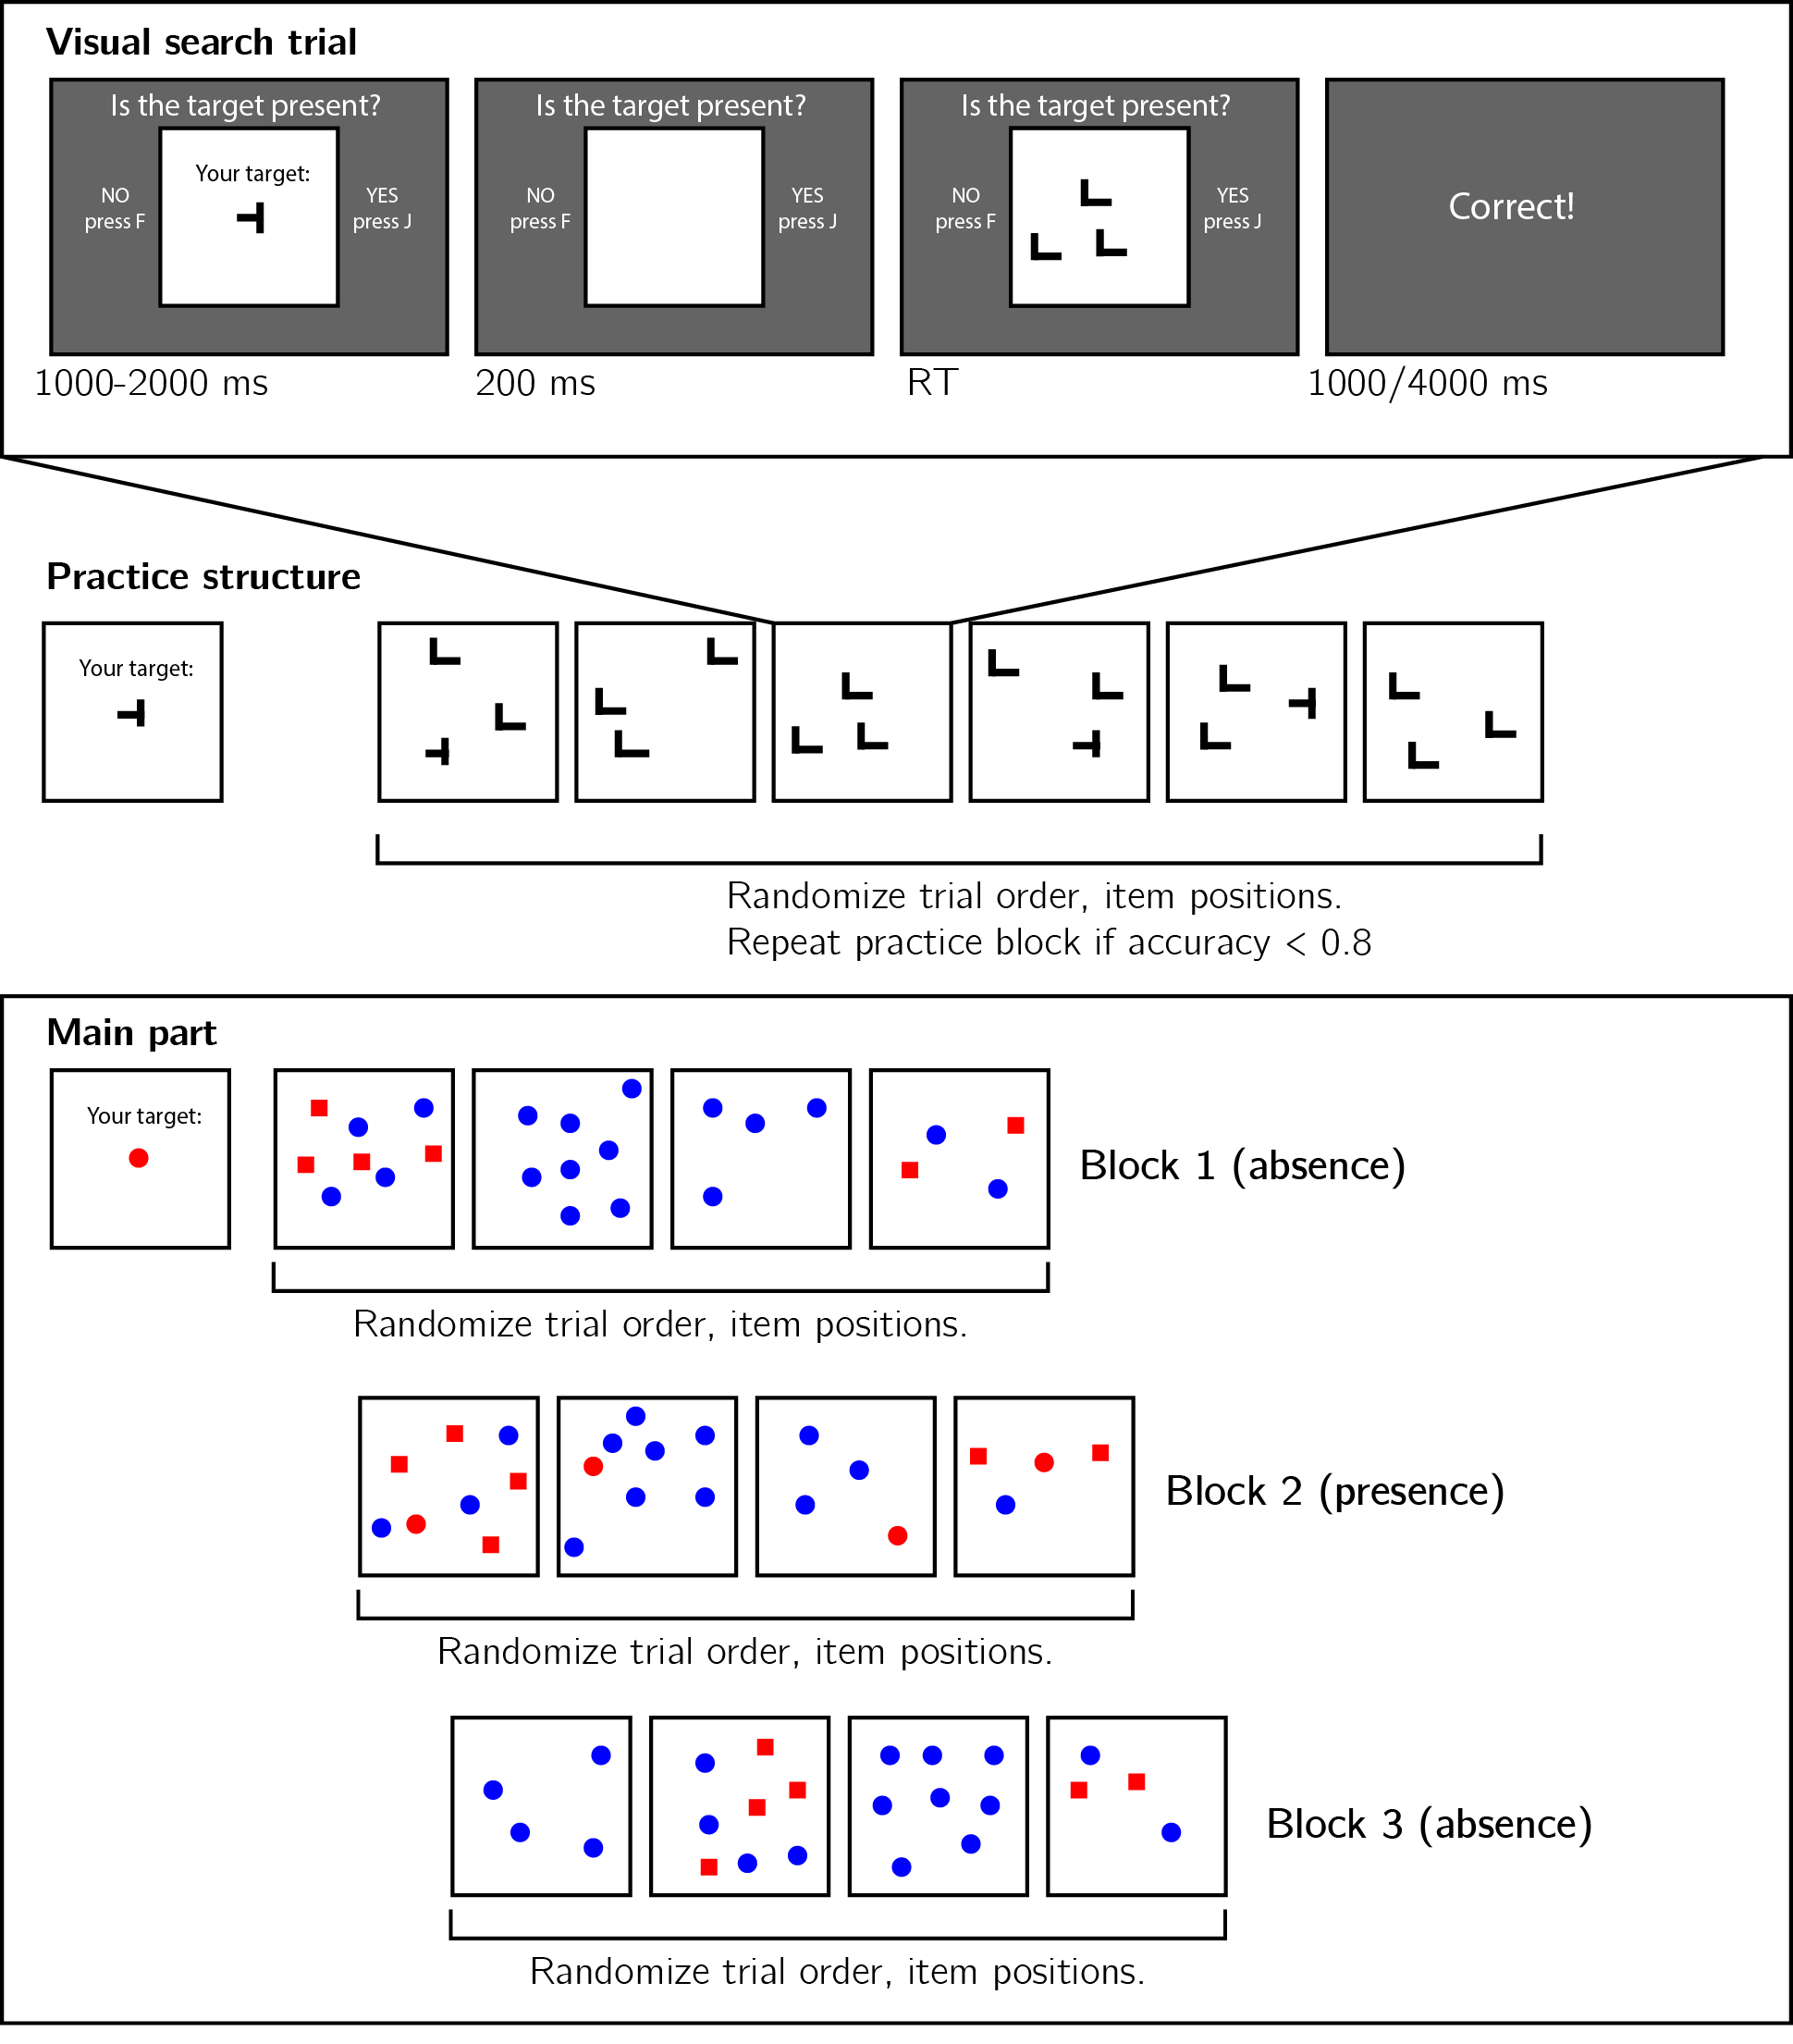
\includegraphics[width=\textwidth]{figures/designExp1} \caption{Experimental design. Top panel: each visual search trial started with a screen indicating the target stimulus. The search display remained visible until a response is recorded. To motivate accurate responses, the feedback screen remained visible for one second following correct responses and for four seconds following errors. Middle panel: after reading the instructions, participants practiced the visual search task in blocks of 6 trials, until they had reached an accuracy level of 0.83 correct or higher (at most one error per block of 6 trials). Bottom panel: the main part of the experiment comprised 12 trials only, in which the target was a red dot. Unbeknown the subjects, only trials 5-8 (Block 2) were target-present trials, and the remaining trials were target-absent trials. Each 4-trial block followed a 2 by 2 design, with factors being set size (4 or 8) and distractor type (color or conjunction; blue dots only or blue dots and red squares, respectively).}\label{fig:design}
\end{figure}

In the main part of the experiment, participants searched for a red dot among blue dots or a mixed array of blue dots and red squares. Set size was set to 4 or 8, resulting in a 2-by-2 design (search type: color or color\(\times\)shape, by set size: 4 or 8). Critically, and unbeknown to subjects, the first four trials were always target-absent trials (one of each set-size \(\times\) search-type combination), presented in randomized order. These trials were followed by the four corresponding target-present trials, presented in randomized order. The final four trials were again target-absent trials, presented in randomized order.

\hypertarget{randomization}{%
\subsubsection{Randomization}\label{randomization}}

The order and timing of experimental events was determined pseudo-randomly by the Mersenne Twister pseudorandom number generator, initialized in a way that ensures registration time-locking (Mazor, Mazor, \& Mukamel, 2019).

\hypertarget{data-analysis}{%
\subsection{Data analysis}\label{data-analysis}}

\hypertarget{rejection-criteria}{%
\subsubsection{Rejection criteria}\label{rejection-criteria}}

Participants were excluded for making more than one error in the main part of the experiment, or for having extremely fast or slow reaction times in one or more of the tasks (below 250 milliseconds or above 5 seconds in more than 25\% of the trials).

Error trials, and trials with response times below 250 milliseconds or above 1 second were excluded from the response-time analysis. All pre-registered analyses without RT-based exclusion are reported in appendix A.

\hypertarget{data-preprocessing}{%
\subsubsection{Data preprocessing}\label{data-preprocessing}}

To control for within-block trial order effects, a linear regression model was fitted separately for each block and participant, predicting search time as a function of trial serial order within the block (\(RT \sim \beta_0+\beta_1i\), with \(i\) denoting the mean-centered serial position within a block). Search times were corrected by subtracting the product of the slope and the mean-centered serial position, in a block-wise manner.

Subject-wise search slopes were then extracted for each combination of search type (color or conjunction) and block number by fitting a linear regression model to the reaction time data with one intercept and one set-size term.

\hypertarget{hypotheses-and-analysis-plan}{%
\subsubsection{Hypotheses and analysis plan}\label{hypotheses-and-analysis-plan}}

Experiment 1 was designed to test several hypotheses about the contribution of metacognitive knowledge to search termination, the state of this knowledge prior to engaging with the task, and the effect of experience trials on this metacognitive knowledge. The specifics of our pre-registered analysis can be accessed in the following link: \url{https://osf.io/ea385}. We outline some possible search time patterns and their pre-registered interpretation in Fig. \ref{fig:models}.

\begin{figure}
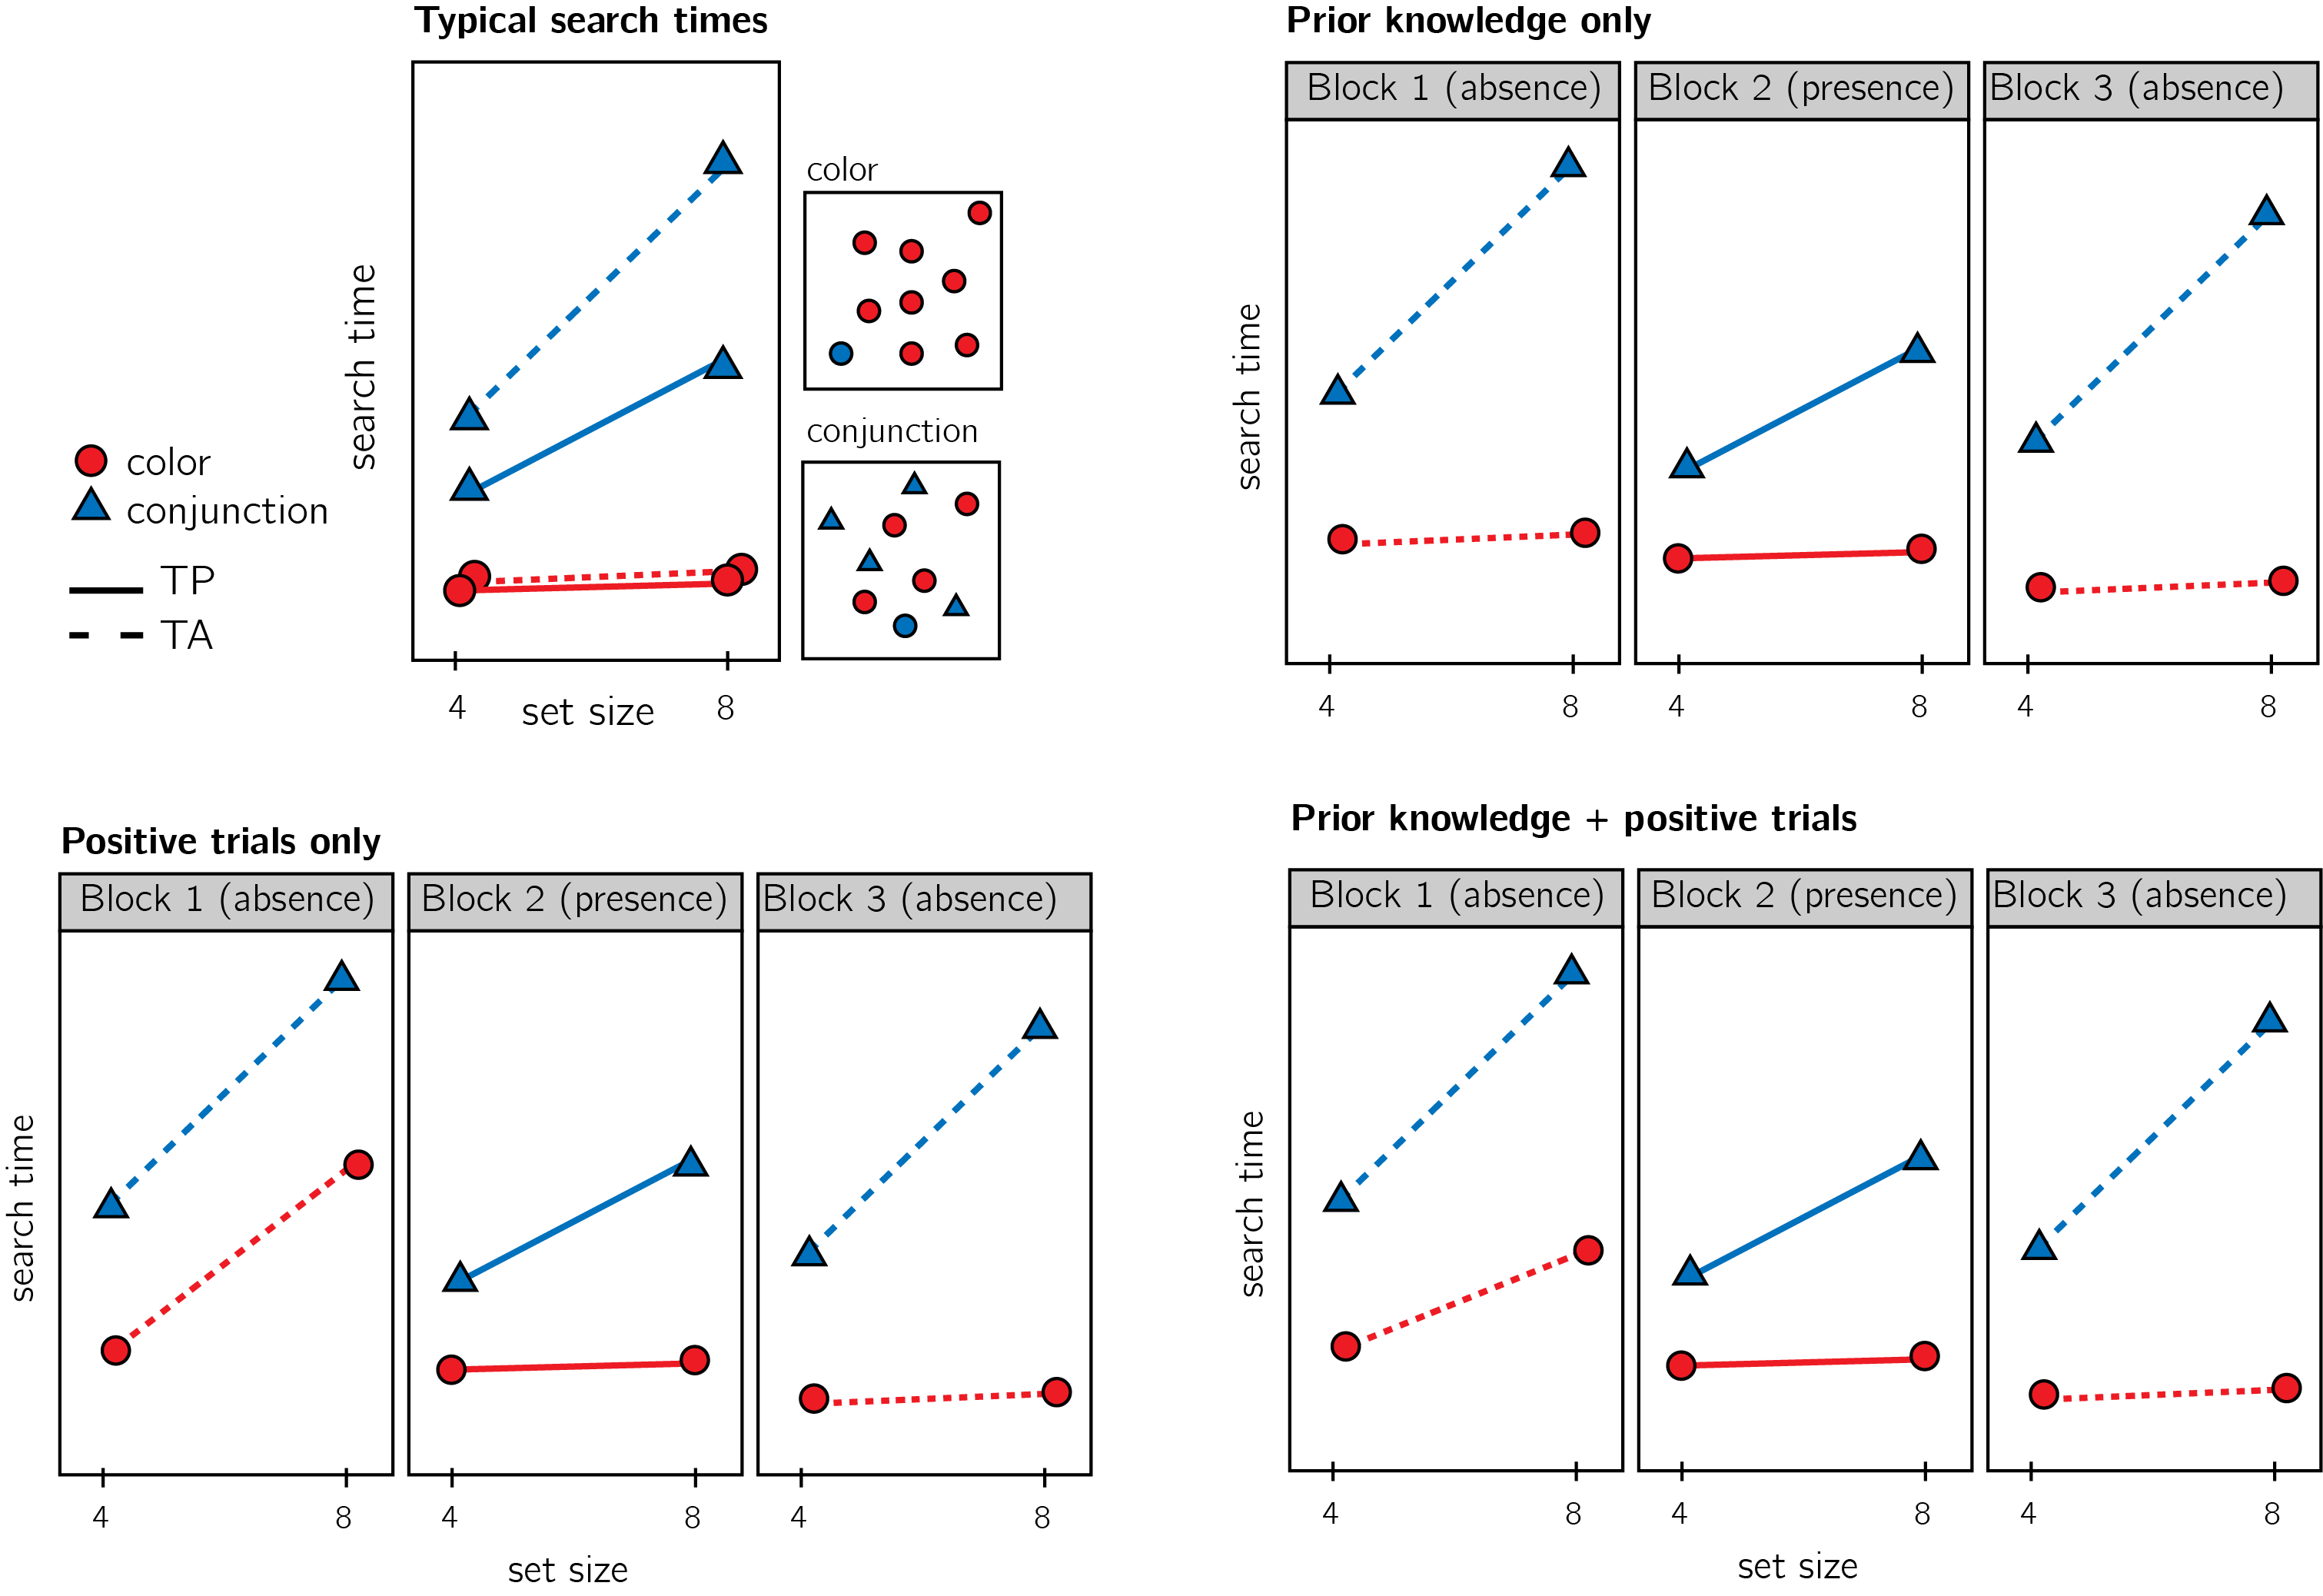
\includegraphics[width=\textwidth]{figures/models} \caption{Visualization of Hypotheses. Top left: typical search time results in visual search experiments with many trials (where TP =  Target Present responses; TA = Target Absent responses). Set size (x axis) affects search time in conjunction search, but much less so in color search. However, it is unclear whether this pattern of target-absent search also holds in the first trials in an experiment. Different models make different predictions about target-absent search times in the first block of the experiment. Top right: one possible pattern is that the same qualitative pattern will be observed in our design, with an overall decrease in response time as a function of trial number. This would suggest that the metacognitive knowledge necessary to support efficient inference about absence was already in place before engaging with the task. Bottom left: an alternative pattern is that the same qualitative pattern will be observed for blocks 2 and 3, but not in block 1. This would suggest that for inference about absence to be efficient, participants had to first experience some target-present trials. Bottom right: alternatively, some degree of metacognitive knowledge may be available prior to engaging with the task, with some being acquired by subsequent exposure to target-present trials. This would manifest as different slopes for conjunction and color searches in blocks 1 and a learning effect for color search between blocks 1 and 3.}\label{fig:models}
\end{figure}

Analysis comprised a positive control based on target-present trials, a test of the presence of a pop-out effect for target-absent color search in block 1, and a test for the change in slope for target-absent color search between blocks 1 and 3. All hypotheses were tested using a within-subject t-test, with a significance level of 0.05.
Given the fact that we only have one trial per cell, one excluded trial is sufficient to make some hypotheses impossible to test on a given participant. For this reason, for each hypothesis separately, participants were included only if all necessary trials met our inclusion criteria. This meant that some hypotheses were tested on different subsets of participants.

We used R (Version 3.6.0; R Core Team, 2019) and the R-packages \emph{BayesFactor} (Version 0.9.12.4.2; Morey \& Rouder, 2018), \emph{cowplot} (Version 1.0.0; Wilke, 2019), \emph{dplyr} (Version 1.0.4; Wickham et al., 2020), \emph{ggplot2} (Version 3.3.1; Wickham, 2016), \emph{jsonlite} (Version 1.7.1; Ooms, 2014), \emph{lsr} (Version 0.5; Navarro, 2015), \emph{MESS} (Version 0.5.6; Ekstrøm, 2019), \emph{papaja} (Version 0.1.0.9997; Aust \& Barth, 2020, 2020, 2020), \emph{pwr} (Version 1.3.0; Champely, 2020), and \emph{tidyr} (Version 1.1.0; Wickham \& Henry, 2020) for all our analyses.

\hypertarget{results}{%
\subsection{Results}\label{results}}

Overall mean accuracy was 0.95 (standard deviation =0.06). Median reaction time was 623.98 ms (median absolute deviation = 127.37). In all further analyses, only correct trials with response times between 250 and 1000 ms are included.

\emph{Hypothesis 1 (positive control)}: Search times in block 2 (target-present) followed the expected pattern, with a steep slope for conjunction search (\(M = 12.52\), 95\% CI \([10.08\), \(14.95]\)) and a shallow slope for color search (\(M = 3.91\), 95\% CI \([2.13\), \(5.70]\); see middle panel in Fig. \ref{fig:exp1Plot}). The slope for color search was significantly lower than 10 ms/item and thus met our criterion for being considered \enquote{pop-out} (\(t(961) = -6.69\), \(p < .001\)). Furthermore, the difference between the slopes was significant (\(t(749) = 6.50\), \(p < .001\)). This positive control served to validate our method of using two trials per participant for obtaining reliable group-level estimates of search slopes.

\emph{Hypothesis 2}: Our central focus was on results from block 1 (target-absent). Here participants didn't yet have experience with searching for the red dot. Similar to the second block, the slope for the conjunction search was steep (\(M = 18.41\), 95\% CI \([14.95\), \(21.87]\)). A clear \enquote{pop-out} effect for color search was also evident (\(M = 0.15\), 95\% CI \([-\infty\), \(2.31]\), \(t(886) = -7.51\), \(p < .001\)). Furthermore, the average search slope for color search in this first block was significantly different from that of the conjunction search (\(t(413) = 6.55\), \(p < .001\); see leftmost panel in Fig. \ref{fig:exp1Plot}), indicating that a color-absence pop-out is already in place prior to direct task experience. This result is in line with the \emph{prior-knowledge only} model (see Fig. \ref{fig:models}), in which participants have valid expectations for efficient color search, prior to engaging with a task.

Pre-registered hypotheses 3-5 were designed to test for a learning effect between blocks 1 and 3, before and after experience with observing a red target among blue distractors. Given the overwhelming pop-out effect for target-absent trials in block 1, not much room for additional learning remained. Indeed, results from these tests support a prior-knowledge only model.

\emph{Hypothesis 3}: Like in the first block, in the third block color search complied with our criterion for \enquote{pop-out} (\(M = 2.27\), 95\% CI \([-\infty\), \(3.86]\), \(t(979) = -7.98\), \(p < .001\)), and was significantly different from the conjunction search slope (\(t(745) = 11.16\), \(p < .001\); see rightmost panel in Fig. \ref{fig:exp1Plot}). This result is not surprising, given that a pop-out effect was already observed in block 1.

\emph{Hypothesis 4}: To quantify the learning effect for color search, we directly contrasted the search slope for color search in blocks 1 and 3. We find no evidence for a learning effect (\(t(799) = -1.15\), \(p = .250\)). Furthermore, a Bayesian t-test with a scaled Cauchy prior for effect sizes (r=0.707) provided strong evidence in favour of the absence of a learning effect (\(\mathrm{BF}_{\textrm{01}} = 12.98\)).

\emph{Hypothesis 5}: In case of a learning effect for pop-out search, Hypothesis 5 was designed to test the specificity of this effect to color pop-out by computing an interaction between block number and search type. Given that no learning effect was observed, this test makes little sense. For completeness, we report that the change in slope between blocks 1 and 3 was similar for color and conjunction search (\(M = -3.58\), 95\% CI \([-10.52\), \(3.36]\), \(t(320) = -1.01\), \(p = .311\)).

\begin{figure}[H]
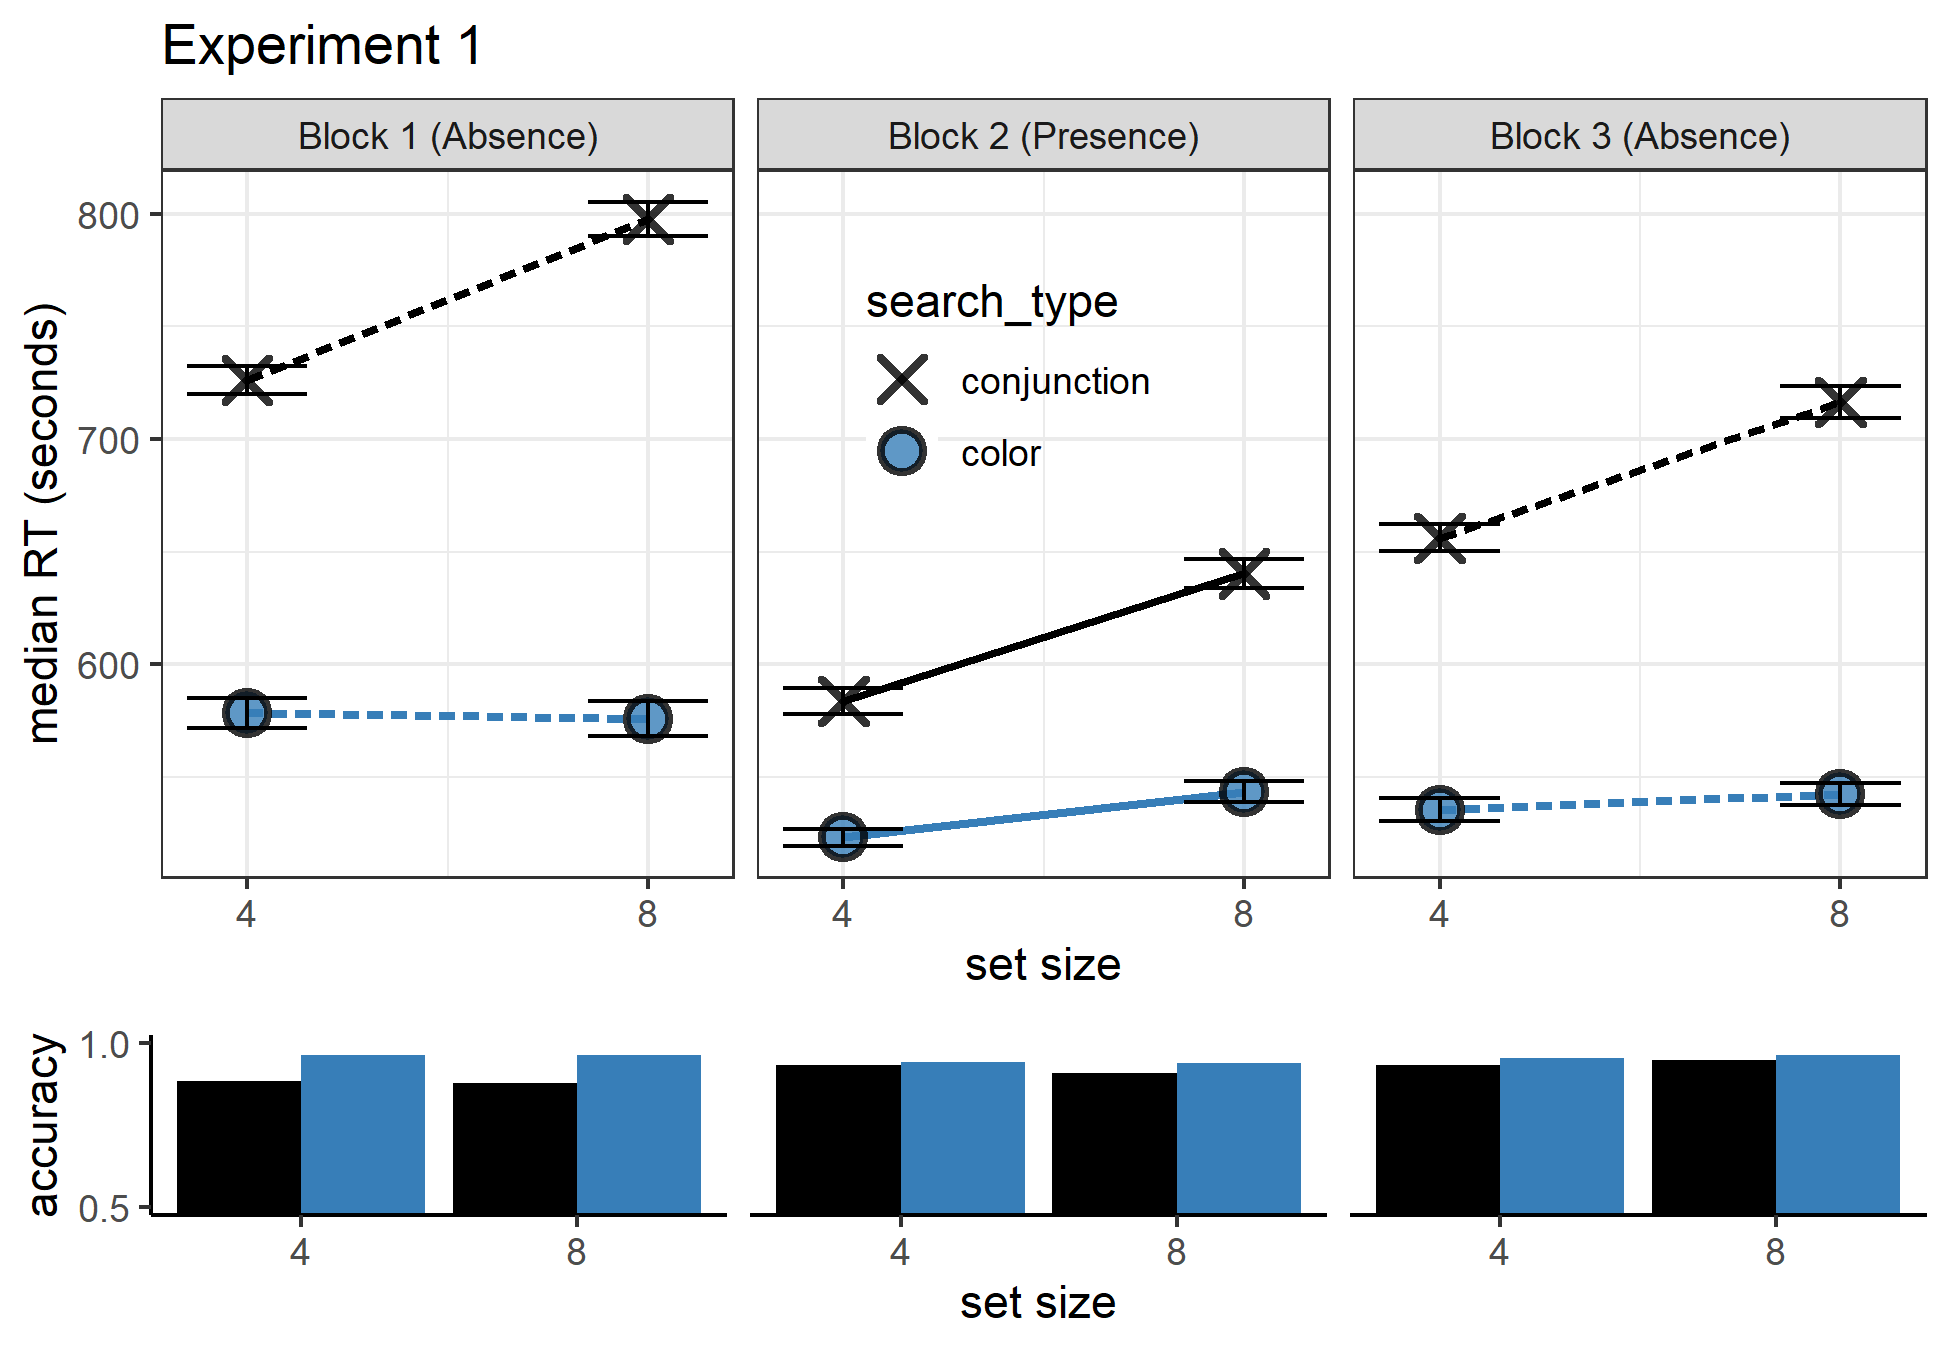
\includegraphics[width=\textwidth]{termination_files/figure-latex/exp1Plot-1} \caption{Upper panel: median search time by distractor set size for the two search tasks across the three blocks (12 trials per participant). Correct responses only. Lower panel: accuracy as a function of block, set size and search type. Error bars represent the standard error of the median (estimated with bootstrapping).}\label{fig:exp1Plot}
\end{figure}

\hypertarget{additional-analyses}{%
\subsection{Additional analyses}\label{additional-analyses}}

\hypertarget{first-trial-only}{%
\subsubsection{First trial only}\label{first-trial-only}}

We considered the possibility that our results do not reflect true zero-shot search termination, but participants' ability to rapidly adjust their termination times based on feedback from previous trials, even within the four trials of the first block. To rule out such within-block learning effects, we tested whether participants showed a color-absence pop-out effect on the very first trial of the experiment. To this end, we analyzed response times in the first trial of the experiment as a function of search type (conjunction or color) and set-size. Since these first trials were slower overall (median RT in the first trial: 881.30 ms compared to 630.34 ms in the last trial), for this exploratory analysis we did not exclude trials based on response times.

Even in this between-subject analysis, with one trial per participant, we found a significant positive search slope for conjunction search (42.75 ms/item, \(p<0.005\)), but not for color search (-12.27 ms/item, \(p=0.43\)). The difference in slopes between conjunction and color, quantified as the interaction between set size and search type in a two-way betwee-subject analysis of variance, was also significant (\(F(1, 1,041) = 6.74\), \(\mathit{MSE} = 466,761.60\), \(p = .010\), \(\hat{\eta}^2_G = .006\); see Fig. \ref{fig:FirstTrial}A). In other words, participants showed a color-absence pop-out already in the first trial of the experiment.

\hypertarget{experiment-2}{%
\section{Experiment 2}\label{experiment-2}}

Experiment 1 provided unequivocal evidence that color-absence pop-out occurs prior to experiencing color pop-out in the context of the same task. We interpret this as indicating that task-naive adults had valid implicit or explicit metacognitive expectations about color pop-out. Experiment 2 was designed to extend these findings to another stimulus feature that is found to also efficiently guide attention: shape. The time cost of additional distractors in shape search was under 10 ms in our pilot data, rendering it another case of parallel, efficient search. It is possible however that unlike in the case of color, the metacognitive knowledge that gives rise to the pop-out effect for shape-absence is acquired through experience with the task. Unlike the colour space, that spans three dimensions only, the space of possible shapes is relatively unconstrained such that having prior knowledge of the expected effect of different shapes on attention requires a richer mental model of attentional processes. Furthrmore, colour is agreed to be a \enquote{guiding attribute of attention}, while it is unclear which shape features guide attention (Wolfe \& Horowitz, 2017). In this experiment we also include an additional control for prior experience with visual search tasks, and ask whether the implicit metacognitive knowledge about pop-out is available for explicit report.

\hypertarget{participants-1}{%
\subsection{Participants}\label{participants-1}}

The research complied with all relevant ethical regulations, and was approved by the Research Ethics Committee of University College London (study ID number 1260/003). 887 Participants were recruited via Prolific, and gave their informed consent prior to their participation. They were selected based on their acceptance rate (\textgreater95\%) and for being native English speakers. We collected data until we reached 320 included participants for hypotheses 1-4 (after applying our pre-registered exclusion criteria). The entire experiment took around 4 minutes to complete (median completion time in our pilot data: 3.93 minutes). Participants were paid £0.51 for their participation, equivalent to an hourly wage of £7.78.

\hypertarget{procedure-1}{%
\subsection{Procedure}\label{procedure-1}}

A static version of Experiment 2 can be accessed on \href{matanmazor.github.io/termination/experiments/demos/exp1/}{matanmazor.github.io/termination/experiments/demos/exp2/}. Experiment 2 was identical to Experiment 1 with the following exceptions. First, instead of color search trials, we included shape search trials, where the red dot target is present or absent in an array of red squares. Second, to minimize the similarity between conjunction and shape searches, conjunction trials included blue dots and red triangles as distractors. Third, to test participants' explicit metacognition about their visual search behaviour, upon completing the main part of the task participants were presented with the four target-absent displays (shape and conjunction displays with 4 or 8 items), and were asked to sort them from fastest to slowest. Finally, participants reported whether they had participated in a similar experiment before, where they were asked to search for shapes on the screen. Participants who responded \enquote{yes} were asked to tell us more about this previous experiment. This question was included in order to examine whether efficient target-absent search in trial 1 reflects prior experience with similar visual search experiments.

Our pre-registered analysis plan for Experiment 2, including rejection criteria and data preprocessing, was identical to our analysis plan for Experiment 1, and can be accessed in the following link: \url{https://osf.io/v6mnb}.

\hypertarget{results-1}{%
\subsection{Results}\label{results-1}}

Overall mean accuracy was 0.96 (standard deviation =0.06). Median reaction time was 644.60 ms (median absolute deviation = 123.89). In all further analyses, only correct trials with response times between 250 and 1000 ms are included.

\emph{Hypothesis 1 (positive control)}: Search times in block 2 (target-present) followed the expected pattern, with a steep slope for conjunction search (\(M = 15.08\), 95\% CI \([12.34\), \(17.83]\)) and a shallow slope for shape search (\(M = 5.84\), 95\% CI \([3.90\), \(7.78]\); see middle panel of Fig. \ref{fig:exp2Plot}). The slope for shape search was significantly lower than 10 ms/item and thus met our criterion for being considered \enquote{pop-out} (\(t(754) = -4.21\), \(p < .001\)). Furthermore, the difference between the slopes was significant (\(t(584) = 4.98\), \(p < .001\)).

\emph{Hypothesis 2}: Our central focus was on results from block 1 (target-absent). Here participants didn't yet have experience with finding the red dot. Similar to the second block, the slope for conjunction search was steep (\(M = 19.53\), 95\% CI \([16.03\), \(23.04]\)). The slope for shape search was numerically lower than 10 ms/item, but not significantly so (\(M = 8.03\), 95\% CI \([-\infty\), \(10.50]\), \(t(608) = -1.31\), \(p = .095\)). Still, the average search slope for shape search in this first block was significantly different from that of the conjunction search (\(t(326) = 2.77\), \(p = .006\); see leftmost panel of Fig. \ref{fig:exp2Plot}), indicating that a processing advantage for the detecting the absence of a shape compared to the absence of shape-color conjunction was already in place before experience with target presence.

Moreover, this processing advantage was not different from what is expected based on shape search slope in block 2 (target presence). A conservative estimate for the ratio between target absence and target presence search slopes is 2 (Wolfe, 1998). Based on this ratio of 2 and the observed target-presence search slope of 6 ms/item, target absence search slope is expected to be 12 ms/item, or higher. Indeed, search slope for shape absence was not significantly different from, and numerically lower than, twice the search slope for shape presence as measured in block 2 (\(t(548) = -1.25\), \(p = .210\)). In other words, our failure to find a pop-out effect for shape absence was not due to participants being suboptimal in their quitting times, but because shape search is indeed more difficult than color search

\emph{Hypothesis 3}: As in the first block, in the third block the slope for shape search was numerically lower than 10 ms/item, but not significantly so (\(M = 8.85\), 95\% CI \([-\infty\), \(10.68]\), \(t(723) = -1.03\), \(p = .151\)). Importantly, the slope for shape search in block 3 was significantly different from the the slope for conjunction search (\(t(565) = 6.02\), \(p < .001\)) and not significantly different from twice the search slope for shape presence (\(t(511) = -2.70\), \(p = .007\); see rightmost panel of Fig. \ref{fig:exp2Plot}).

\emph{Hypothesis 4}: To quantify a potential learning effect for shape search between blocks 1 and 3, we directly contrasted the search slope for shape search in these two \enquote{target-absent} blocks. We find no evidence for a learning effect (\(t(542) = -0.03\), \(p = .974\)). Furthermore, a Bayesian t-test with a scaled Cauchy prior for effect sizes (r=0.707) provided strong evidence against a learning effect (\(\mathrm{BF}_{\textrm{01}} = 20.72\)). Like in Experiment 1, these results are most consistent with a \emph{prior-knowledge only} model (see Fig. \ref{fig:models}), in which participants already know to expect that shape search should be easier than conjunction search, prior to having direct experience with target-present trials.

\begin{figure}[H]
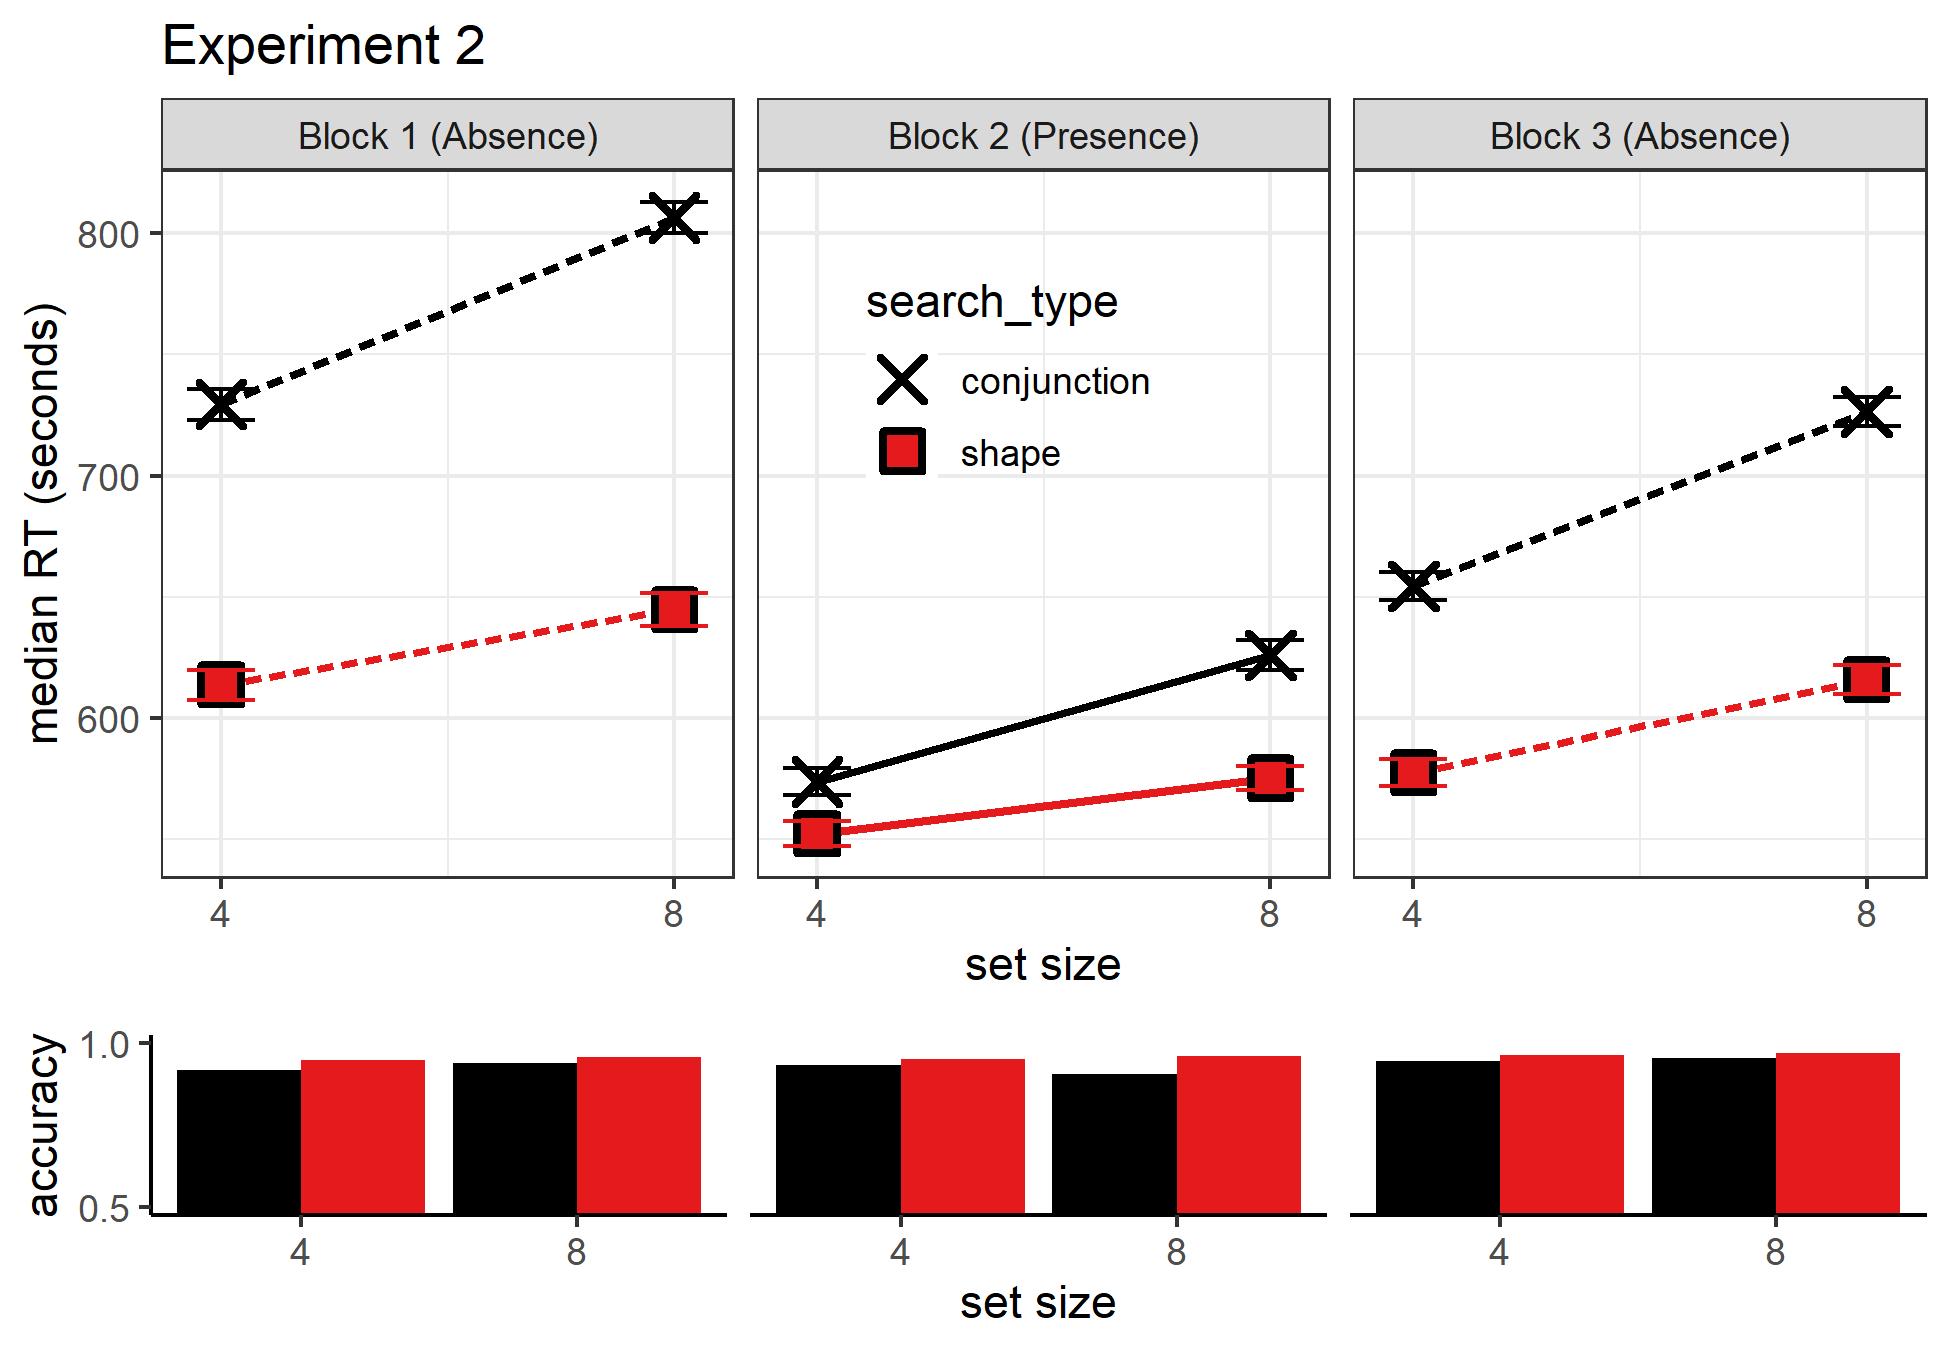
\includegraphics[width=\textwidth]{termination_files/figure-latex/exp2Plot-1} \caption{Upper panel: median search time by distractor set size for the two search tasks across the three blocks. Correct responses only. Lower panel: accuracy as a function of block, set size and search type. Error bars represent the standard error of the median (estimated with bootstrapping).}\label{fig:exp2Plot}
\end{figure}

\hypertarget{additional-analyses-1}{%
\subsection{Additional Analyses}\label{additional-analyses-1}}

\hypertarget{first-trial-only-1}{%
\subsubsection{First trial only}\label{first-trial-only-1}}

Like in Exp. 1, here also we followed up on our pre-registered analysis with an exploratory between-subject analysis, focusing on the first trials only. Here also, we observed a significant positive search slope for conjunction search (43.65 ms/item, \(p<0.0005\)), but not for shape search (9.80 ms/item, \(p=0.40\)). The difference in slopes between conjunction and shape, quantified as the interaction between set size and search type in a two-way betwee-subject analysis of variance, was significant (\(F(1, 781) = 4.25\), \(\mathit{MSE} = 209,989.78\), \(p = .040\), \(\hat{\eta}^2_G = .005\); see Fig. \ref{fig:FirstTrial}B).

\begin{figure}[H]
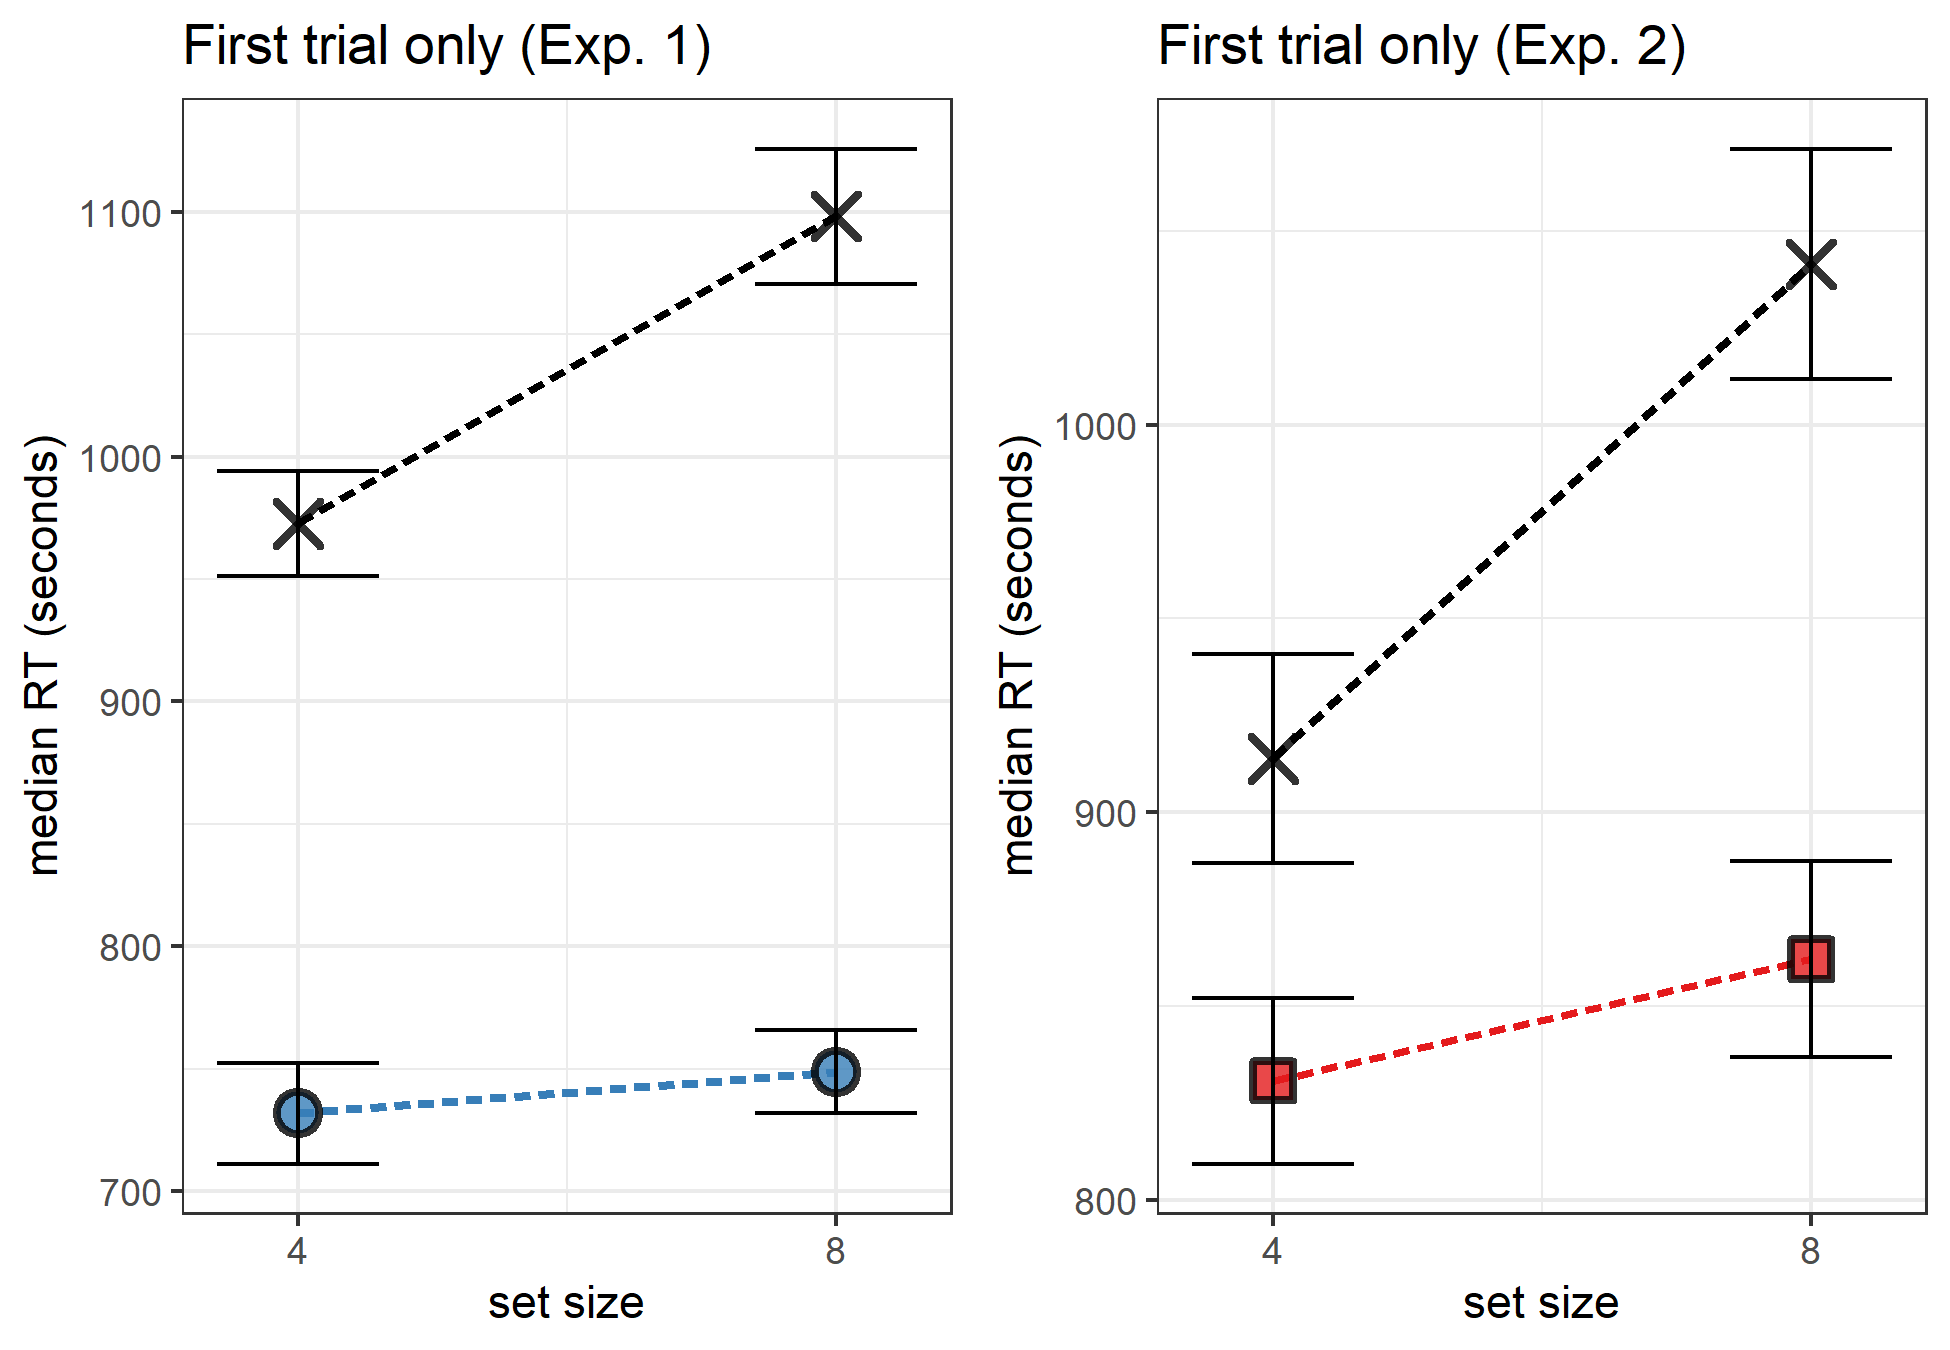
\includegraphics[width=\textwidth]{termination_files/figure-latex/FirstTrial-1} \caption{Median search time by distractor set size for Experiments 1 and 2, looking at the first trial of each participant only. Error bars represent the standard error of the median (estimated with bootstrapping).}\label{fig:FirstTrial}
\end{figure}

\hypertarget{exploratory-analysis-task-experience}{%
\subsection{Exploratory analysis: task experience}\label{exploratory-analysis-task-experience}}

At the end of the experiment, participants were asked if they have ever participated in a similar experiment before, where they were asked to search for a target item. 796 participants answered \enquote{no} to this question. For those participants, a highly efficient search for a distinct shape in the first trials of the experiment, if found, cannot be due to prior experience performing a visual search task with similar stimuli. Participants that reported having no prior experience with a visual search task still showed efficient search termination for shape distractors (\(M = 7.32\), 95\% CI \([4.21\), \(10.43]\)), and were significantly more efficient in terminating shape search than conjunction search in the first 4 target-absent trials (\(t(296) = 2.68\), \(p = .008\)). Efficient search termination for shape search is therefore not dependent on prior visual search trials, neither within the same experiment nor in previous ones.

\hypertarget{exploratory-analysis-search-time-estimates}{%
\subsection{Exploratory analysis: search time estimates}\label{exploratory-analysis-search-time-estimates}}

Upon completing the main part of Experiment 2, participants placed the four search arrays (shape and conjunction searches with 4 or 8 distractors) on a perceived difficulty axis. We used these ratings to ask whether the advantage for detecting the absence of a distinct shape over the absence of a shape/color conjunction depended on explicit access to metacognitive knowledge about search difficulty. The decision to quit early in target-absent shape search trials may depend on an internal belief that the target shape would have drawn attention immediately, but this belief may be inaccessible to introspection. If introspective access is not a necessary condition for efficient quitting in visual search, some participants may not be able to reliably introspect about the difficulty of different searches but still be able to quit efficiently in shape search.

For this analysis, we only considered the ratings of participants who engaged with the array-sorting trial, and moved some of the arrays before continuing to the next trial (N=789). Searches with 8 distractors were rated as more difficult than searches with 4 distractors, in line with the set-size effect (\(t(788) = 31.62\), \(p < .001\)). Furthermore, conjunction searches were rated as more difficult than shape searches (\(t(788) = 5.11\), \(p < .001\)). Finally, we fitted single-subject linear regression models to the two search types, predicting search-time estimates (the position of each condition on a continuous perceived difficulty scale) as a function of set size. Similar to actual search slopes, these slopes derived from subjective estimates were also shallower for shape than for conjunction search, reflecting a belief that the effect of set size in shape search is not as strong as the effect of set size in conjunction search (\(M = 6.45\), 95\% CI \([2.81\), \(10.08]\), \(t(788) = 3.48\), \(p = .001\)).

Subjective search time estimates revealed that by the end of the experiment, the average participant considered the slope of shape search to be shallower than that of conjunction search. This suggests that at least some participants had introspective access to their visual search behaviour. But were those participants whose estimates reflected a shallow slope for shape search the same ones that were more efficient in detecting the absence of a shape in the display? The slopes of retrospective estimates for shape search were not reliably correlated with actual search slopes for shape absence in block 1 (\(r = .08\), 95\% CI \([-.06\), \(.22]\)) or 2 (\(r = .02\), 95\% CI \([-.12\), \(.16]\)). However, this result should be interpreted carefully in light of the low reliability of single subject estimated that are derived from one trial per cell. Indeed, search slopes for shape absence in blocks 1 and 3 were not reliably correlated themselves (\(r = .05\), 95\% CI \([-.10\), \(.19]\)).

To answer this question using a more severe test (Mayo, 2018), we focused on the subset of participants whose difficulty orderings reflected the erroneous belief that shape search was more difficult than conjunction search (\(N=\) 83). If efficient search termination depends on accurate explicit metacognitive knowledge about search efficiency, search termination in this subset of participants is not expected to be more efficient in shape compared to conjunction search, and is even expected to show the opposite pattern. In contrast with this prediction, and in support of a functional dissociation between explicit and implicit metacognitive knowledge, search slopes for shape-absence trials were shallower than for conjunction-absence trials (\(M_d = 12.45\), 95\% CI \([5.21\), \(19.69]\), \(t(82) = 3.42\), \(p = .001\)).

\hypertarget{discussion}{%
\section{Discussion}\label{discussion}}

Deciding that an item is absent requires counterfactual thinking, in the form of \enquote{I would have seen it if it was present}. In some cases, it is immediately clear that an hypothetical target would have been detected (such as when searching for a red item, but seeing only blue items), and in other cases more deliberate searching is needed until this belief can be held with confidence (such as when searching for a conjunction of features, for example colour and shape). Here we sought to determine the origins of this metacognitive knowledge that allows participants to conclude that a target would be found immediately in the first case, but not in the second. Specifically, we asked if this knowledge depends on task experience (such that with time, participants learn that some searches are easier than others), or alternatively, whether it is available already in the first trials of the experiment.

Previous studies of search termination have focused on the calibration of a quitting strategy over long chains of similar trials. For example, in a seminal study by Chun and Wolfe (1996), participants decreased their activation threshold (the necessary activation for an item to be scanned) following misses, but increased the threshold following correct rejections. This calibration mechanism critically depended on two features of the experimental design: a large number of similar trials, and explicit feedback about accuracy. Similarly, in a multi-session perceptual training study by Ellison and Walsh (1998), response times became faster over sessions, and search slopes for conjunction search became shallower. In more recent studies, participants were able to learn statistical regularities in spatial position (Moorselaar \& Slagter, 2019) and visual features (Moorselaar, Lampers, Cordesius, \& Slagter, 2020) of distractor stimuli in a visual search task, and to use this information for making faster responses. These studies revealed important mechanisms by which task experience can affect visual search behaviour, but they left open the question of what guides search termination in the absence of any task experience. Our zero-shot search termination paradigm revealed that some knowledge about search efficiency is available to participants already in the first trials of the experiment, before engaging with the task or knowing what distractors to expect.

In two experiments, no prior experience with color or shape pop-out in previous trials was needed for participants to be able to terminate the search early when a target was absent. Participants were sensitive to the counterfactual likelihood of detecting a hypothetical target even in the first trials of the experiment, suggesting that metacognitive knowledge about visual attention (e.g., \enquote{red pops out}, or \enquote{a dot would catch my attention}) is available to guide zero-shot search termination. In Experiment 2, we find that some of this knowledge is represented explicitly, as expressed in participants' ordering of visual search arrays by difficulty. However, focusing on participants with erroneous metacognitive beliefs about search efficiency, we find that explicit metacognitive knowledge is not a necessary condition for efficient search termination. More broadly, this finding indicates a functional dissociation between explicit and implicit metacognitive knowledge.

\hypertarget{is-implicit-metacognitive-knowledge-metacognitive}{%
\subsection{Is implicit metacognitive knowledge metacognitive?}\label{is-implicit-metacognitive-knowledge-metacognitive}}

In this study we assumed that efficient search termination is impossible without accurate metacognitive knowledge about search difficulty. We base this conjecture on our conceptual analysis of inference about absence: in order to represent something as absent, one must know that they would have detected it had it been present (Mazor \& Fleming, 2020). Alternative approaches to visual search assume that the absence of a stimulus can sometimes be perceived directly, without alluding to any metacognitive beliefs or counterfactual thinking. For example, ensemble perception allows observers to extract summary statistical information from sets of similar stimuli, without directly perceiving every single stimulus (Whitney \& Yamanashi Leib, 2018). According to one alternative explanation of our results, if participants immediately perceive that the search array is all blue, they might not need to rely on any counterfactual thinking or self-knowledge to conclude that no red item was present. Similarly, when searching for a red dot, there is no need to serially scan a search array if it is immediately perceived as comprising only squares.

When contrasting this alternative account with our counterfactual model, it is useful to ask how does the visual system extract ensemble properties from sets of objects. For the global statistical property \enquote{the array comprises only squares} to be extracted from a display without representing individual squares, the visual system must represent, explicitly or implicitly, that a non-square item would have been detected if present. This representation can be implemented, for example, as a threshold on curvature-sensitive neurons (\enquote{a round object would have induced a higher firing rate in this neuron population}), or more generally as a likelihood function going from polygons to firing patterns (\enquote{The perceived input is most likely under a world state where the display includes polygons only}). Even within the ensemble perception framework, inference about the absence of items must be based on some form of meta-level knowledge about the cognitive and perceptual systems. The fact that attention may not be required for ensemble perception (Hochstein, Pavlovskaya, Bonneh, \& Soroker, 2015) can inform and constrain our theories of where this meta-level knowledge is represented in the cognitive hierarchy, but it does not, by itself, weigh on the question of whether this is indeed metacognitive knowledge.

We note here that it not a prerequisite that metacognitive knowledge be accessible to consciousness. Metacognitive knowledge was originally assumed by Flavell (1979) to mostly affect cognition without accessing consciousness at all (i.e.~without inducing a \enquote{metacognitive experience}). Different aspects of metacognition monitoring, including an immediate \emph{Feeling of Knowing} when presented with a problem, have been attributed to implicit metacognitive mechanisms that share a conceptual similarity with the ones described in the previous paragraph (Reder \& Schunn, 1996). More relevant to visual search, a schematic model of attention has been suggested to be implemented in the brains of many animal species, including all mammals and birds, and to facilitate attention control and monitoring (Graziano, 2013). This \emph{Attention Schema} is metacognitive in the sense that it reflects self knowledge about one's own attention. This kind of implicit metacognitive knowledge may be crucial for extracting ensemble statistics from displays, and for representing the absence of objects.

\hypertarget{inference-about-absence-as-a-tool-for-studying-implicit-self-knowledge}{%
\subsection{Inference about absence as a tool for studying implicit self knowledge}\label{inference-about-absence-as-a-tool-for-studying-implicit-self-knowledge}}

Participants' early quitting in target-absence feature searches taught us something about implicit self-knowledge. This is not a coincidence, but an example of a general principle: inference about absence critically relies on self-knowledge not only in visual search (\enquote{If a target was present, I would have found it}) but also in near-threshold detection (\enquote{If a stimulus was present, I would have noticed it}), recognition memory (\enquote{If this item was in the study list, I would have remembered it}), and problem-solving (\enquote{If a solution to this problem was present, I would have come up with it}). This makes inference about absence an important tool for studying implicit self-knowledge in a range of domains without relying on explicit metacognitive reports. For example, in the context of recognition memory, items that are most likely to be remembered are also the ones that are most likely to be correctly rejected as foils when new. This \enquote{mirror effect} (Brown, Lewis, \& Monk, 1977) conceptually resembles the alignment of feature-present and feature-absent search times across items and visual dimensions in visual search: if a target is found easily within a set of distractors \emph{S}, it would also be easy to conclude that a target is absent if \emph{S} is presented without the target in it. Just as in the study of visual search, previous studies of the mirror effect adopted a typical many subjects/few trials designs (e.g., Brown et al., 1977; Glanzer \& Adams, 1985; Greene \& Thapar, 1994). By generalizing the approach we have taken here to implicit metacognitive knowledge of memory, future \emph{Zero-shot negative recognition} experiments could ask whether the self knowledge that gives rise to the mirror effect is also available prior to engaging with the task.

\hypertarget{conclusion}{%
\subsection{Conclusion}\label{conclusion}}

Search termination in the first few trials of an experiment (zero shot search termination) showed the same qualitative response time pattern as that commonly found in typical (few subjects/many trials) visual search experiments. Given that no target was present in these trials, participants must have been sensitive to the counterfactual likelihood of them finding the target, had it been present. In Experiment 2 we showed that this metacognitive knowledge about search difficulty was often accessible to report, but that this was not a necessary condition for efficient search termination. We interpret our results as indicating a dissociation between implicit and explicit metacognitive knowledge, with the former having a particularly influential role in inference about absence.

\hypertarget{references}{%
\section{References}\label{references}}

\begingroup
\setlength{\parindent}{-0.5in}
\setlength{\leftskip}{0.5in}

\hypertarget{refs}{}
\leavevmode\hypertarget{ref-R-papaja}{}%
Aust, F., \& Barth, M. (2020). \emph{papaja: Create APA manuscripts with R Markdown}. Retrieved from \url{https://github.com/crsh/papaja}

\leavevmode\hypertarget{ref-brown1977memorability}{}%
Brown, J., Lewis, V., \& Monk, A. (1977). Memorability, word frequency and negative recognition. \emph{The Quarterly Journal of Experimental Psychology}, \emph{29}(3), 461--473.

\leavevmode\hypertarget{ref-R-pwr}{}%
Champely, S. (2020). \emph{Pwr: Basic functions for power analysis}. Retrieved from \url{https://CRAN.R-project.org/package=pwr}

\leavevmode\hypertarget{ref-chun1996just}{}%
Chun, M. M., \& Wolfe, J. M. (1996). Just say no: How are visual searches terminated when there is no target present? \emph{Cognitive Psychology}, \emph{30}(1), 39--78.

\leavevmode\hypertarget{ref-d1991color}{}%
D'Zmura, M. (1991). Color in visual search. \emph{Vision Research}, \emph{31}(6), 951--966.

\leavevmode\hypertarget{ref-R-MESS}{}%
Ekstrøm, C. T. (2019). \emph{MESS: Miscellaneous esoteric statistical scripts}. Retrieved from \url{https://CRAN.R-project.org/package=MESS}

\leavevmode\hypertarget{ref-ellison1998perceptual}{}%
Ellison, A., \& Walsh, V. (1998). Perceptual learning in visual search: Some evidence of specificities. \emph{Vision Research}, \emph{38}(3), 333--345.

\leavevmode\hypertarget{ref-flavell1979metacognition}{}%
Flavell, J. H. (1979). Metacognition and cognitive monitoring: A new area of cognitive--developmental inquiry. \emph{American Psychologist}, \emph{34}(10), 906.

\leavevmode\hypertarget{ref-glanzer1985mirror}{}%
Glanzer, M., \& Adams, J. K. (1985). The mirror effect in recognition memory. \emph{Memory \& Cognition}, \emph{13}(1), 8--20.

\leavevmode\hypertarget{ref-graziano2013consciousness}{}%
Graziano, M. S. (2013). \emph{Consciousness and the social brain}. Oxford University Press.

\leavevmode\hypertarget{ref-greene1994mirror}{}%
Greene, R. L., \& Thapar, A. (1994). Mirror effect in frequency discrimination. \emph{Journal of Experimental Psychology: Learning, Memory, and Cognition}, \emph{20}(4), 946.

\leavevmode\hypertarget{ref-hochstein2015global}{}%
Hochstein, S., Pavlovskaya, M., Bonneh, Y. S., \& Soroker, N. (2015). Global statistics are not neglected. \emph{Journal of Vision}, \emph{15}(4), 7--7.

\leavevmode\hypertarget{ref-hulleman2017impending}{}%
Hulleman, J., \& Olivers, C. N. (2017). The impending demise of the item in visual search. \emph{Behavioral and Brain Sciences}, \emph{40}.

\leavevmode\hypertarget{ref-mayo2018statistical}{}%
Mayo, D. G. (2018). \emph{Statistical inference as severe testing}. Cambridge: Cambridge University Press.

\leavevmode\hypertarget{ref-mazor2020distinguishing}{}%
Mazor, M., \& Fleming, S. M. (2020). Distinguishing absence of awareness from awareness of absence. \emph{Philosophy and the Mind Sciences}, \emph{1}(II).

\leavevmode\hypertarget{ref-mazor2019novel}{}%
Mazor, M., Mazor, N., \& Mukamel, R. (2019). A novel tool for time-locking study plans to results. \emph{European Journal of Neuroscience}, \emph{49}(9), 1149--1156.

\leavevmode\hypertarget{ref-van2020neural}{}%
Moorselaar, D. van, Lampers, E., Cordesius, E., \& Slagter, H. A. (2020). Neural mechanisms underlying expectation-dependent inhibition of distracting information. \emph{Elife}, \emph{9}, e61048.

\leavevmode\hypertarget{ref-van2019learning}{}%
Moorselaar, D. van, \& Slagter, H. A. (2019). Learning what is irrelevant or relevant: Expectations facilitate distractor inhibition and target facilitation through distinct neural mechanisms. \emph{Journal of Neuroscience}, \emph{39}(35), 6953--6967.

\leavevmode\hypertarget{ref-moran2013competitive}{}%
Moran, R., Zehetleitner, M., Müller, H. J., \& Usher, M. (2013). Competitive guided search: Meeting the challenge of benchmark rt distributions. \emph{Journal of Vision}, \emph{13}(8), 24--24.

\leavevmode\hypertarget{ref-R-BayesFactor}{}%
Morey, R. D., \& Rouder, J. N. (2018). \emph{BayesFactor: Computation of bayes factors for common designs}. Retrieved from \url{https://CRAN.R-project.org/package=BayesFactor}

\leavevmode\hypertarget{ref-R-lsr}{}%
Navarro, D. (2015). \emph{Learning statistics with r: A tutorial for psychology students and other beginners. (Version 0.5)}. Adelaide, Australia: University of Adelaide. Retrieved from \url{http://ua.edu.au/ccs/teaching/lsr}

\leavevmode\hypertarget{ref-R-jsonlite}{}%
Ooms, J. (2014). The jsonlite package: A practical and consistent mapping between json data and r objects. \emph{arXiv:1403.2805 {[}stat.CO{]}}. Retrieved from \url{https://arxiv.org/abs/1403.2805}

\leavevmode\hypertarget{ref-R-base}{}%
R Core Team. (2019). \emph{R: A language and environment for statistical computing}. Vienna, Austria: R Foundation for Statistical Computing. Retrieved from \url{https://www.R-project.org/}

\leavevmode\hypertarget{ref-reder1996metacognition}{}%
Reder, L. M., \& Schunn, C. D. (1996). Metacognition does not imply awareness: Strategy choice is governed by implicit learning and memory.

\leavevmode\hypertarget{ref-treisman1980feature}{}%
Treisman, A. M., \& Gelade, G. (1980). A feature-integration theory of attention. \emph{Cognitive Psychology}, \emph{12}(1), 97--136.

\leavevmode\hypertarget{ref-whitney2018ensemble}{}%
Whitney, D., \& Yamanashi Leib, A. (2018). Ensemble perception. \emph{Annual Review of Psychology}, \emph{69}, 105--129.

\leavevmode\hypertarget{ref-R-ggplot2}{}%
Wickham, H. (2016). \emph{Ggplot2: Elegant graphics for data analysis}. Springer-Verlag New York. Retrieved from \url{https://ggplot2.tidyverse.org}

\leavevmode\hypertarget{ref-R-dplyr}{}%
Wickham, H., François, R., Henry, L., \& Müller, K. (2020). \emph{Dplyr: A grammar of data manipulation}. Retrieved from \url{https://CRAN.R-project.org/package=dplyr}

\leavevmode\hypertarget{ref-R-tidyr}{}%
Wickham, H., \& Henry, L. (2020). \emph{Tidyr: Tidy messy data}. Retrieved from \url{https://CRAN.R-project.org/package=tidyr}

\leavevmode\hypertarget{ref-R-cowplot}{}%
Wilke, C. O. (2019). \emph{Cowplot: Streamlined plot theme and plot annotations for 'ggplot2'}. Retrieved from \url{https://CRAN.R-project.org/package=cowplot}

\leavevmode\hypertarget{ref-wolfe2021guided}{}%
Wolfe, J. (2021). Guided search 6.0: An updated model of visual search. \emph{Psychonomic Bulletin \& Review}.

\leavevmode\hypertarget{ref-wolfe2012quit}{}%
Wolfe, J. M. (2012). When do i quit? The search termination problem in visual search. \emph{The Influence of Attention, Learning, and Motivation on Visual Search}, 183--208.

\leavevmode\hypertarget{ref-wolfe2007guided}{}%
Wolfe, J. M., \& Gray, W. (2007). Guided search 4.0. \emph{Integrated Models of Cognitive Systems}, 99--119.

\leavevmode\hypertarget{ref-wolfe2017five}{}%
Wolfe, J. M., \& Horowitz, T. S. (2017). Five factors that guide attention in visual search. \emph{Nature Human Behaviour}, \emph{1}(3), 1--8.

\endgroup


\end{document}
